\documentclass[11pt,a4paper]{article}
\usepackage{notes}
\usepackage{tikz}
\usetikzlibrary{decorations.pathmorphing, arrows.meta} % for snake/wavy lines
\usepackage{amsmath}
\usepackage{fancyhdr}
\usepackage{multicol}

\pagestyle{fancy}
\fancyhf{}
\lhead{Geophysics IIIA: Potential Fields \& Geothermics}
\rhead{Week 5 Ocean--Continent Problem}
\cfoot{\thepage}

\title{Week 5 --- Isostasy Problem:\\ Oceanic vs Continental Crust}
\author{Geophysics 3A: Potential Fields \& Geothermics}
\date{\today}

\begin{document}
\maketitle

\section*{Part A: Crust-only Airy Isostasy}

\textbf{Given:}
\begin{multicols}{2}
\begin{description}[itemsep=0.0em, topsep=0.5em]
    \item [oceanic crust thickness:] $h_{oc} = \SI{7}{km}$
    \item [ocean depth:] $h_w = \SI{3.7}{km}$
    \item [seawater density:] $\rho_w = \SI{1030}{\du}$
    \item [continental crust thickness:] $h_{cc} = \SI{40}{km}$
    \item [continental crust density:] $\rho_{cc} = \SI{2850}{\du}$
    \item [continental elevation:] $\varepsilon = \SI{0.8}{km}$
    \item [mantle density:] $\rho_a = \SI{3330}{\du}$
\end{description}
\end{multicols}

\textbf{Instructions:}  
Assume isostatic compensation occurs solely through crustal thickness. Compute the density of the oceanic crust, $\rho_{oc}$, that balances the oceanic and continental columns. Compare your result with typical oceanic crust densities (\(\sim\)2900--3000~\du) and discuss why the crust-only assumption may fail.

\begin{figure}[h!]
    \centering
    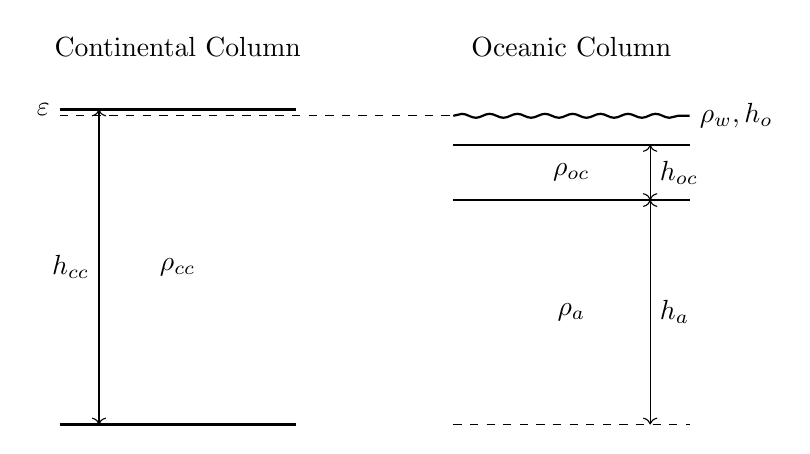
\begin{tikzpicture}[scale=0.1]

    \def\hcc{40}
    \def\elev{0.8}
    \def\hoc{7}
    \def\hw{3.7}

    % --- Continental column ---
    % Continental crust top (elevation h_c)
    \draw[thick] (0,\hcc) -- (30,\hcc);
    % Continental crust base
    \draw[thick] (0,0) -- (30,0);

    \node[left] at (0,\hcc) {$\varepsilon$};
    \draw[dashed] (0,\hcc-\elev) -- (50,\hcc-\elev);

    % --- Oceanic column ---
    % Mantle root below ocean (Airy root)
    \draw[dashed] (50,0) -- (80,0);
    % Oceanic crust base
    \draw[thick] (50,\hcc-\elev-\hw-\hoc) -- (80,\hcc-\elev-\hw-\hoc);
    % Oceanic crust top
    \draw[thick] (50,\hcc-\elev-\hw) -- (80,\hcc-\elev-\hw);
    % Water surface above ocean
    \draw[thick, decorate, decoration={snake, amplitude=0.25mm}] 
    (50,\hcc-\elev) -- (80,\hcc-\elev) node[right]{$\rho_w, h_o$};

    % --- Labels ---
    \node at (15,1.2*\hcc) {Continental Column};
    \node at (65,1.2*\hcc) {Oceanic Column};

    % --- Thickness arrows ---
    \draw[<->] (5,0) -- (5,\hcc) node[midway,left]{$h_{cc}$};
    \draw[<->] (75,\hcc-\elev-\hw) -- (75,\hcc-\elev-\hw-\hoc) node[midway,right]{$h_{oc}$};
    \draw[<->] (75,\hcc-\elev-\hw-\hoc) -- (75,0) node[midway,right]{$h_a$};

    % --- Density labels ---
    \node at (15,20) {$\rho_{cc}$};
    \node at (65,\hcc-\elev-\hw-\hoc/2) {$\rho_{oc}$};
    \node at (65,\hcc/2-\elev/2-\hw/2-\hoc/2) {$\rho_a$};

    \end{tikzpicture}
    \caption{Comparision of isostatic columns for the continental and oceanic crust for Part A.}
    \label{fig:partA}
\end{figure}

\textbf{Questions:}
\begin{enumerate}
    \item Compute the required oceanic crust density $\rho_{oc}$.
    \item Compare with expected oceanic crust densities and discuss why the simple crust-only model may not yield realistic values.
\end{enumerate}

\section*{Part B: Two-layer Lithosphere Model}

\textbf{Given additional information:}
\begin{description}[topsep=0.5em,itemsep=0.0em]
    \item [Oceanic lithospheric mantle thickness] $h_{om} = \SI{75}{km}$
    \item [Oceanic lithospheric mantle density:] $\rho_{om} = \SI{3330}{\du}$
    \item [Continental lithospheric mantle thickness:] $h_{cm} = \SI{150}{km}$
    \item [Continental lithospheric mantle density:] $\rho_{cm} =\ ?$
    \item [Asthenosphere density:] $\rho_a = \SI{3320}{\du}$
\end{description}

\textbf{Instructions:}  
Let's add a two-layered lithosphere using average lithospheric thicknesses for the oceanic and continental settings.  Our goal will be to see what we can learn about the relative density difference between continental and oceanic mantle lithosphere.  In the process, we'll show how including the mantle lithosphere resolves the unrealistic crust-only result.

\begin{figure}[h!]
    \centering
    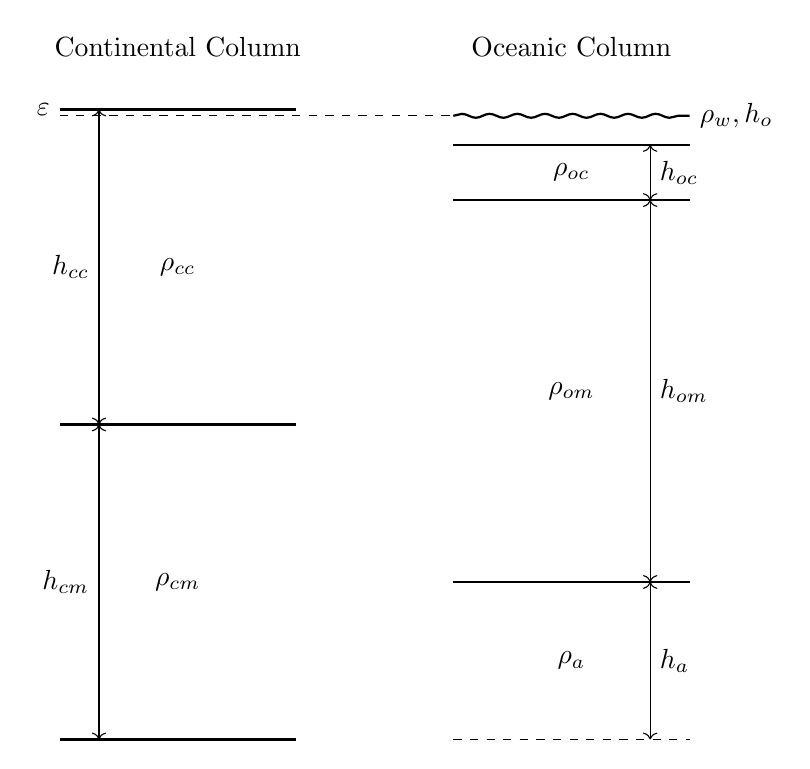
\begin{tikzpicture}[scale=0.1]

    \def\hcc{40}
    \def\elev{0.8}
    \def\hoc{7}
    \def\hw{3.7}
    \def\hcm{-40}
    \def\hom{-20}

    % --- Continental column ---
    % Continental crust top (elevation h_c)
    \draw[thick] (0,\hcc) -- (30,\hcc);
    % Continental crust base
    \draw[thick] (0,0) -- (30,0);
    % Continental lithosphere
    \draw[thick] (0,\hcm) -- (30,\hcm);

    \node[left] at (0,\hcc) {$\varepsilon$};
    \draw[dashed] (0,\hcc-\elev) -- (50,\hcc-\elev);

    % --- Oceanic column ---
    % Oceanic crust base
    \draw[thick] (50,\hcc-\elev-\hw-\hoc) -- (80,\hcc-\elev-\hw-\hoc);
    % Oceanic crust top
    \draw[thick] (50,\hcc-\elev-\hw) -- (80,\hcc-\elev-\hw);
    % Water surface above ocean
    \draw[thick, decorate, decoration={snake, amplitude=0.25mm}] 
    (50,\hcc-\elev) -- (80,\hcc-\elev) node[right]{$\rho_w, h_o$};
    % Mantle lithosphere
    \draw[thick] (50,\hom) -- (80,\hom);
    % Mantle root below ocean (Airy root)
    \draw[dashed] (50,\hcm) -- (80,\hcm);

    % --- Labels ---
    \node at (15,1.2*\hcc) {Continental Column};
    \node at (65,1.2*\hcc) {Oceanic Column};

    % --- Thickness arrows ---
    \draw[<->] (5,0) -- (5,\hcc) node[midway,left]{$h_{cc}$};
    \draw[<->] (5,0) -- (5,\hcm) node[midway,left]{$h_{cm}$};

    \draw[<->] (75,\hcc-\elev-\hw) -- (75,\hcc-\elev-\hw-\hoc) node[midway,right]{$h_{oc}$};
    \draw[<->] (75,\hcc-\elev-\hw-\hoc) -- (75,\hom) node[midway,right]{$h_{om}$};
    \draw[<->] (75,\hom) -- (75,\hcm) node[midway,right]{$h_a$};

    % --- Density labels ---
    \node at (15,20) {$\rho_{cc}$};
    \node at (15,\hcm/2) {$\rho_{cm}$};
    \node at (65,\hcc-\elev-\hw-\hoc/2) {$\rho_{oc}$};
    \node at (65,\hom+\hcc/2-\elev/2-\hw/2-\hoc/2-\hom/2) {$\rho_{om}$};
    \node at (65,\hom+\hcm/2-\hom/2) {$\rho_a$};

    \end{tikzpicture}
    \caption{Comparision of isostatic columns for the continental and oceanic crust for Part B.}
    \label{fig:partB}
\end{figure}

\begin{table}[h!]
    \centering
    \caption{Modal proportions of minerals in the oceanic and continental lithospheres.}
    \label{tab:modes}
    \begin{tabular}{lcc}
        \toprule
        \textbf{Mineral} &
        \textbf{Oceanic} &
        \textbf{Continental} \\
        \midrule
        olivine & 75 & 60 \\
        orthopyroxene & 25 & 17 \\
        clinopyroxene & 10 & 11 \\
        garnet & 0 & 12 \\
        \bottomrule
    \end{tabular}
\end{table}
\FloatBarrier

Oceanic lithospheric mantle is assumed to be composed of depleted peridotite with a density of \(\rho_{om} = \SI{3330}{\du}\). Continental lithospheric mantle may contain a higher proportion of garnet.

\begin{description}[itemsep=0.0em, topsep=0.5em]
    \item [Density of depleted mantle (peridotite):] \(\rho_d = \SI{3330}{\du}\)
    \item [Density of garnet:] \(\rho_g = \SI{3600}{\du}\)
\end{description}

\textbf{Questions:}
\begin{enumerate}
    \item Setup the isostatic equations for a two-layered mantle lithosphere.  If we assume an average oceanic crustal density $\rho_{oc} = $2900--3000~\du, what density of the continental mantle lithopshere?

    \item Explain how including the mantle lithosphere resolves the unrealistic density obtained in the crust-only case.

    \item Discuss the role of garnet fraction in the continental lithospheric mantle for the density contrast. Compute the percentage difference garnet between the oceanic and continental lithsophere and compare your result with the modal proportions in Table~\ref{tab:modes}.
\end{enumerate}

\end{document}